\lstinputlisting[language=bash,basicstyle=\small]{python_codes/fieldstone_112/keywords}

\begin{center}
\inpython~Code at \url{https://github.com/cedrict/fieldstone/tree/master/python_codes/fieldstone_112}
\end{center}

\par\noindent\rule{\textwidth}{0.4pt}

%%%%%%%%%%%%%%%%%%%%%%%%%%%%%%%%%%%%%%%%%%%%%%%%%%%%%%%%%%%%%%%%%%%%%%%%%%%%%%%%%%%%%%%%%%%%%%%%%%%%

This \stone showcases the MINI (Section~\ref{pair:mini}), 
$P_2\times P_1$ (Section~\ref{ss:p2p1}), $Q_2\times Q_1$ (Section~\ref{ss:pairq2q1}), 
$Q_2\times P_{-1}$ (Section~\ref{ss:pairq2pm1} - unmapped approach, see \stone~76) 
and Crouzeix-Raviart  (Section~\ref{sec:crouzeix-raviart}) elements.
All experiments take place in the unit square (except SolVg). 

The mesh is composed of $nel_x \times nel_y$ cells which are cut in half via the same 
diagonal (NW-SE) into 2 triangles for simplicity\footnote{I revisit this for SolVi} 
when triangular elements are used: 

\begin{center}

\includegraphics[width=7cm]{python_codes/fieldstone_112/results/exp1/grid_quads}

\includegraphics[width=7cm]{python_codes/fieldstone_112/results/exp1/grid_triangles}\\
{\captionfont Quadrilaterals and triangles mesh for a resolution of $16\times 16$ cells.} 
\end{center}

The last pressure dof is fixed to remove the nullspace and the obtained pressure field
is then normalised so that $\int_\Omega p dV = 0$.

Resolutions are ranging from $8\times 8$ to maximum $320\times320$. The high resolution runs take hours 
because python is slow. $320\times 320$ seems to be the limit on my 32Gb-RAM laptop (I build and feed 
the entire Stokes matrix to the solver).  

These are the important numerical parameters which allow to control the type of calculation in the code:
\begin{itemize}
\item {\tt elt}=MINI, P2P1, CR, Q2Q1 or Q2P1.
\item {\tt experiment}: 1$\rightarrow$ Donea \& Huerta manufactured solution;
2 $\rightarrow$ high viscosity sinker; 3$\rightarrow$ SolCx; 4$\rightarrow$ SolCx; 
5$\rightarrow$ SolVi; 6$\rightarrow$ SolVg (viscosity grooves).
\item {\tt nelx,nely}:  the number of cells in each direction
\item {\tt randomize\_mesh} allows to add a small random perturbation to the nodes
\end{itemize}

\newpage
%========================================================
\subsection*{Donea \& Huerta manufactured solution}

We start with the manufactured solution problem "Donea \& Huerta" (see Section~\ref{mms1}).

\begin{center}
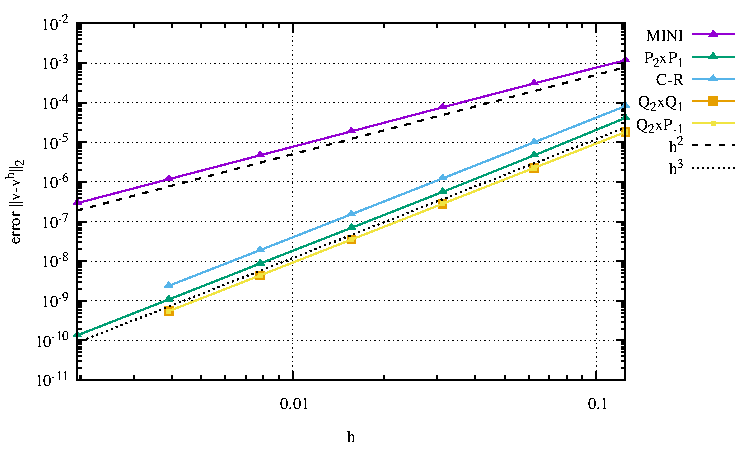
\includegraphics[width=8cm]{python_codes/fieldstone_112/results/exp1/errors_V.pdf}
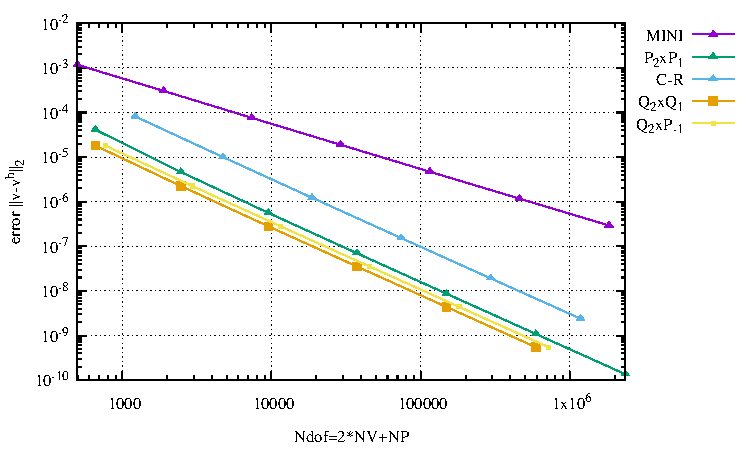
\includegraphics[width=8cm]{python_codes/fieldstone_112/results/exp1/errors_V_ndof.pdf}\\
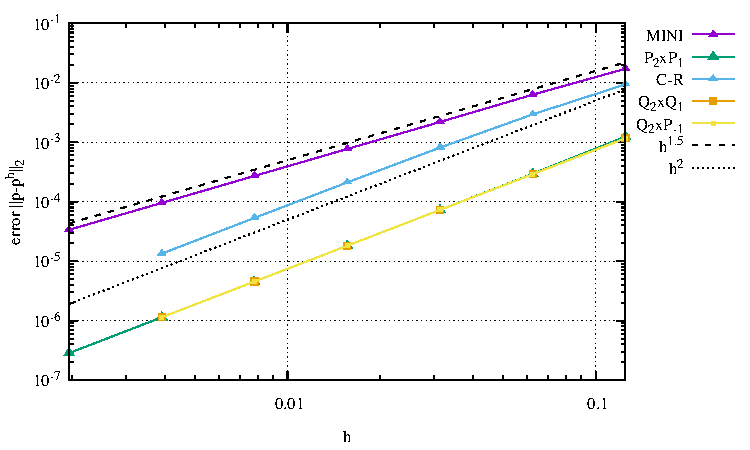
\includegraphics[width=8cm]{python_codes/fieldstone_112/results/exp1/errors_P.pdf}
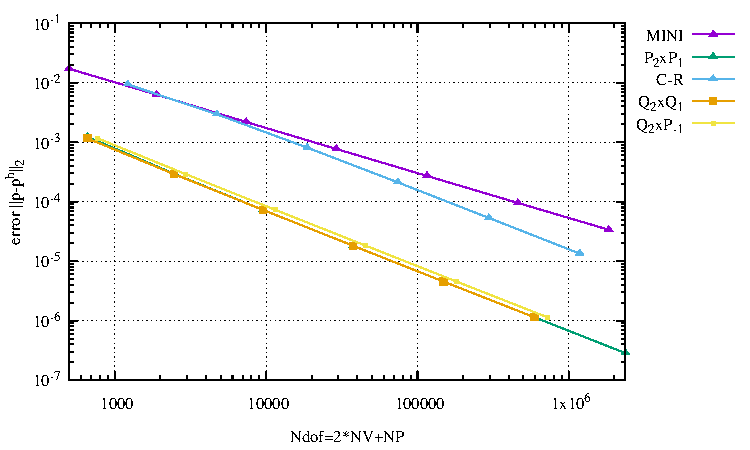
\includegraphics[width=8cm]{python_codes/fieldstone_112/results/exp1/errors_P_ndof.pdf}\\
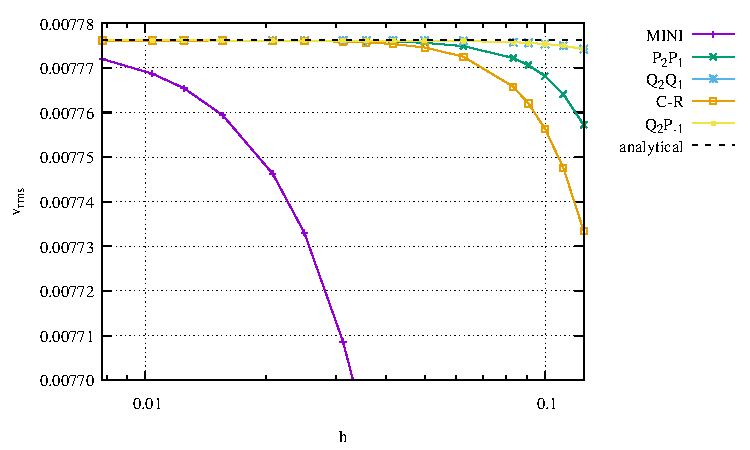
\includegraphics[width=8cm]{python_codes/fieldstone_112/results/exp1/vrms.pdf}
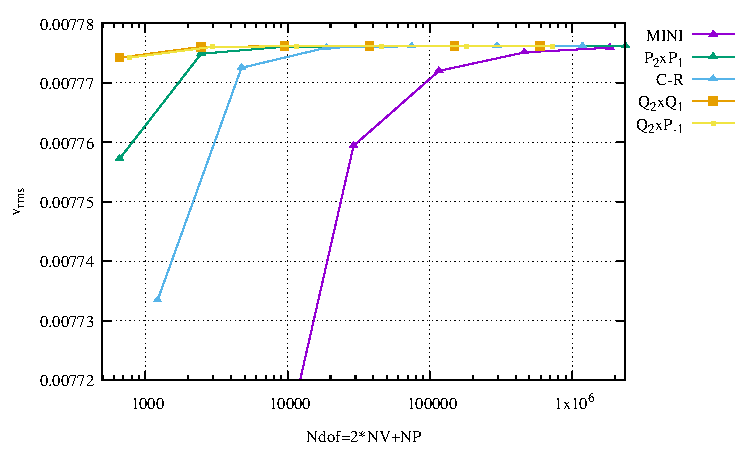
\includegraphics[width=8cm]{python_codes/fieldstone_112/results/exp1/vrms_ndof.pdf}\\
{\captionfont Velocity $L_2$ error (top row), pressure $L_2$ error (middle row) and root
mean square velocity (bottom row) as a function of the element size $h$ (left column) 
and the total number of degrees of freedom (right column).}
\end{center}

\newpage
\begin{center}
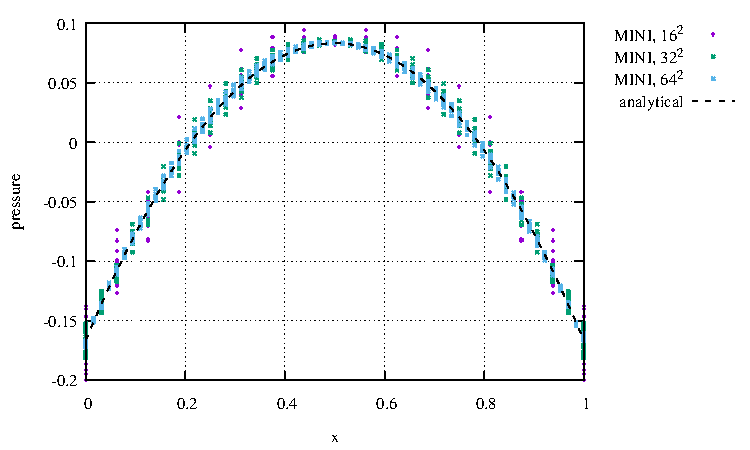
\includegraphics[width=8.5cm]{python_codes/fieldstone_112/results/exp1/pressMINI}
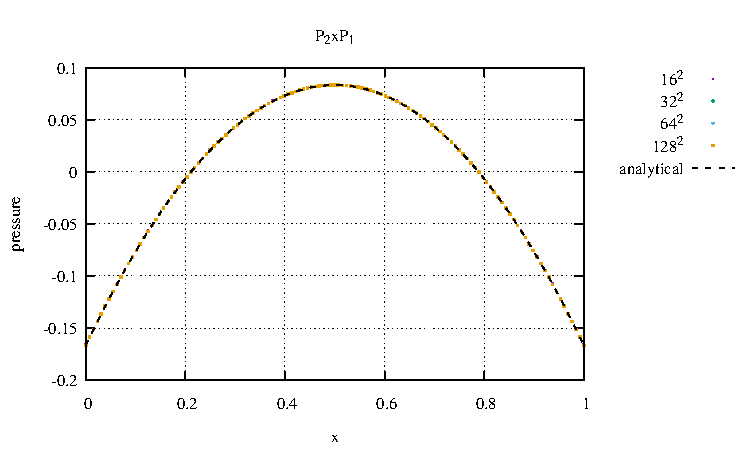
\includegraphics[width=8.5cm]{python_codes/fieldstone_112/results/exp1/pressP2P1}\\
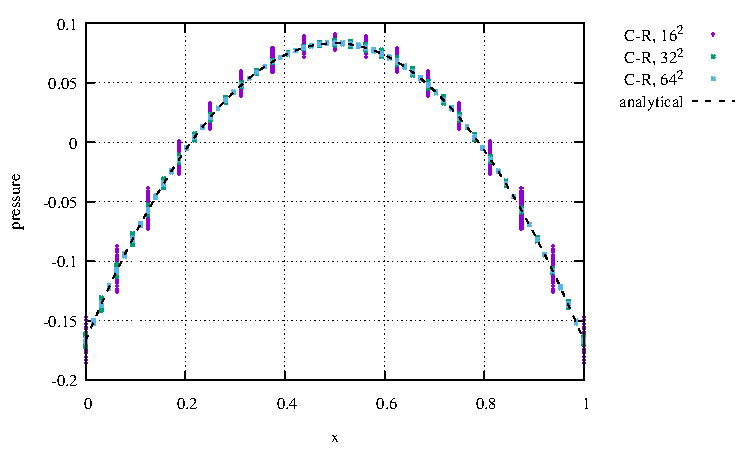
\includegraphics[width=8.5cm]{python_codes/fieldstone_112/results/exp1/pressCR}
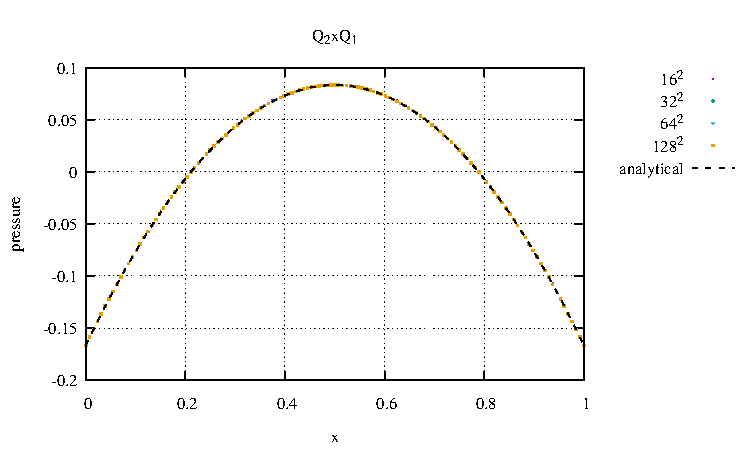
\includegraphics[width=8.5cm]{python_codes/fieldstone_112/results/exp1/pressQ2Q1}\\
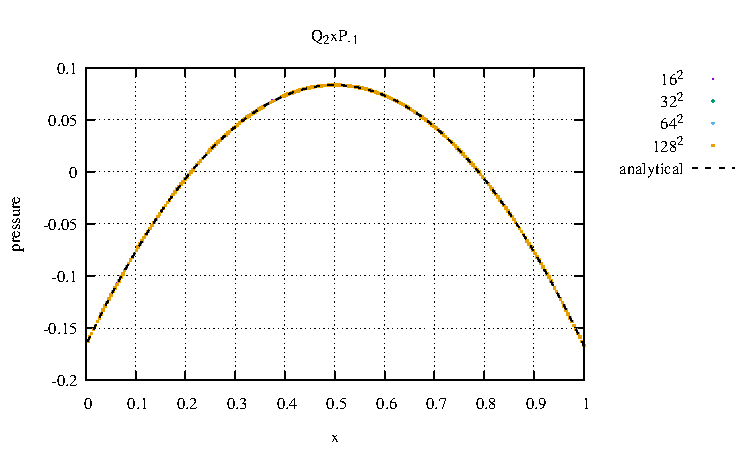
\includegraphics[width=8.5cm]{python_codes/fieldstone_112/results/exp1/pressQ2P1}\\
{\captionfont Pressure field as a function of the $x$-coordinate on a $16\times16$,
$32\times 32$ and $64\times 64$ mesh for all 5 elements.} 
\end{center}

\newpage

Influence of mesh quality:
A random perturbation is added to the interior nodes. 

\begin{center}
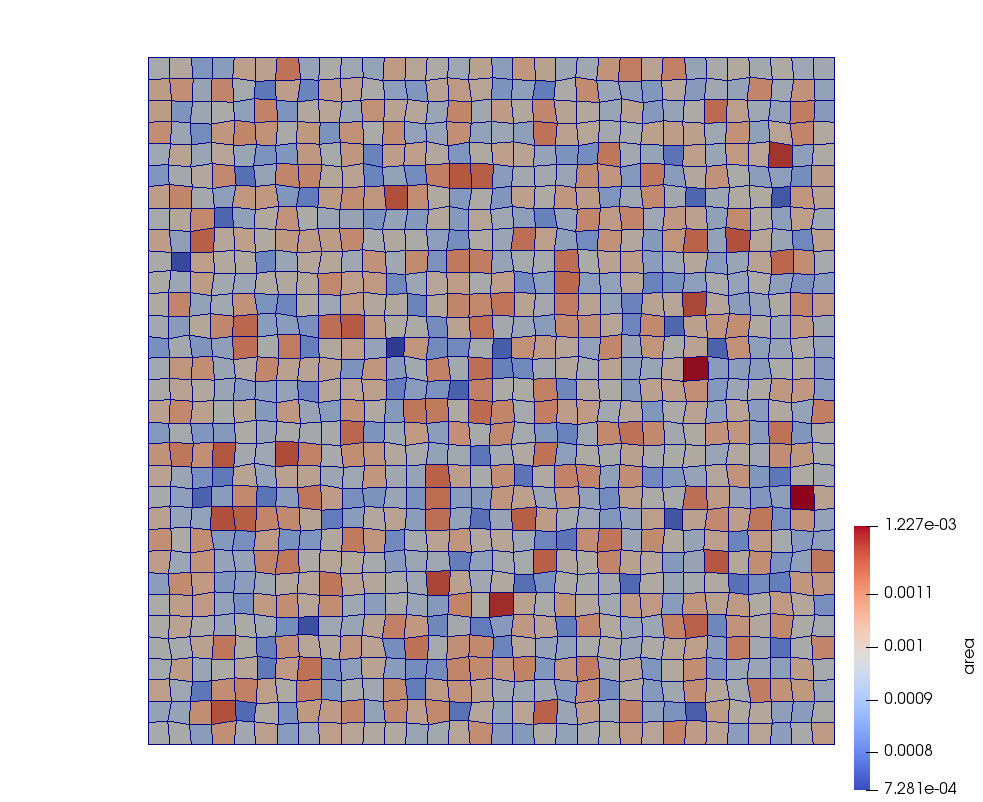
\includegraphics[width=6cm]{python_codes/fieldstone_112/results/exp1_rand/area_quads}
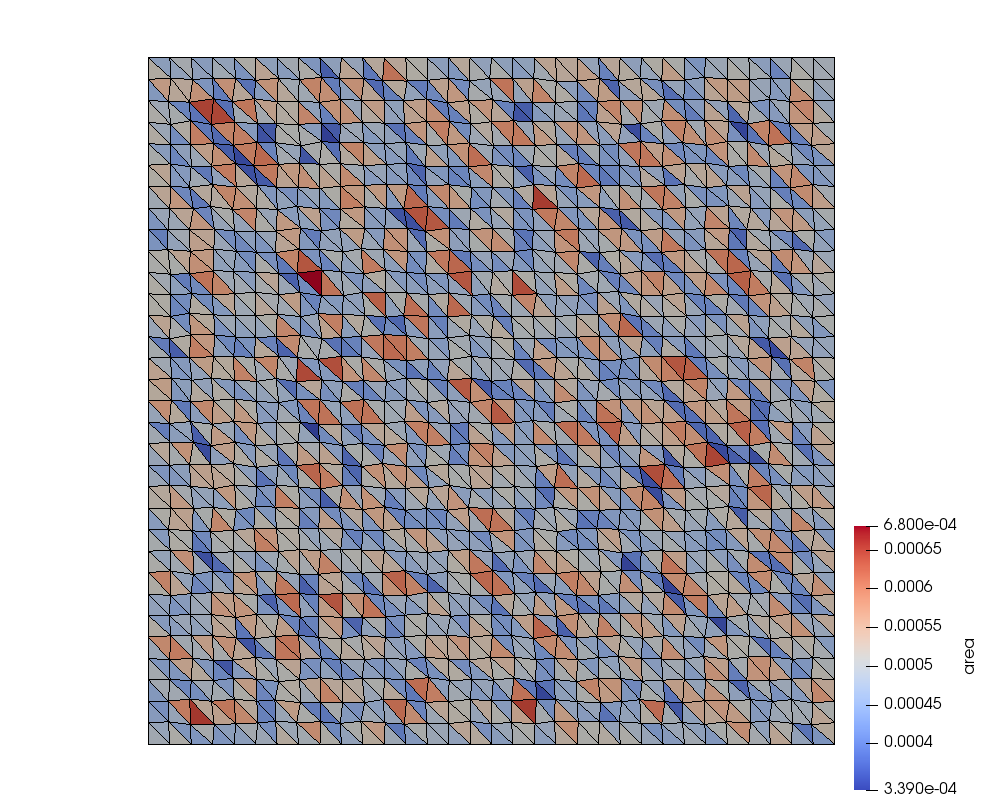
\includegraphics[width=6cm]{python_codes/fieldstone_112/results/exp1_rand/area_tris}\\
{\captionfont Mesh and element areas for quadrilaterals and triangles on a 32x32 cell mesh.}
\end{center}

\begin{center}
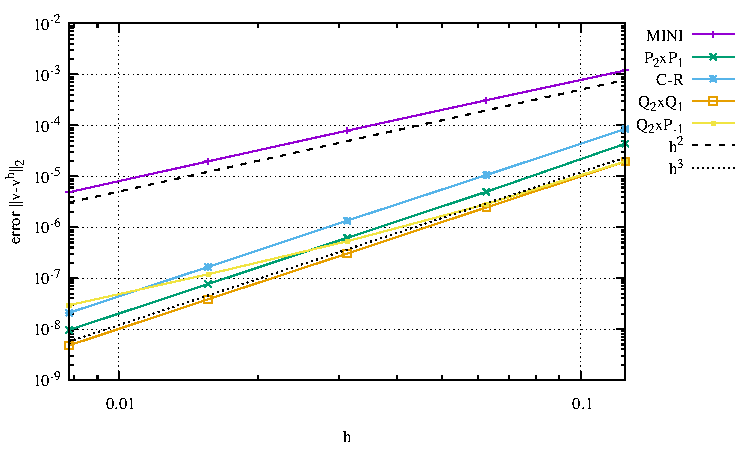
\includegraphics[width=8cm]{python_codes/fieldstone_112/results/exp1_rand/errors_V.pdf}
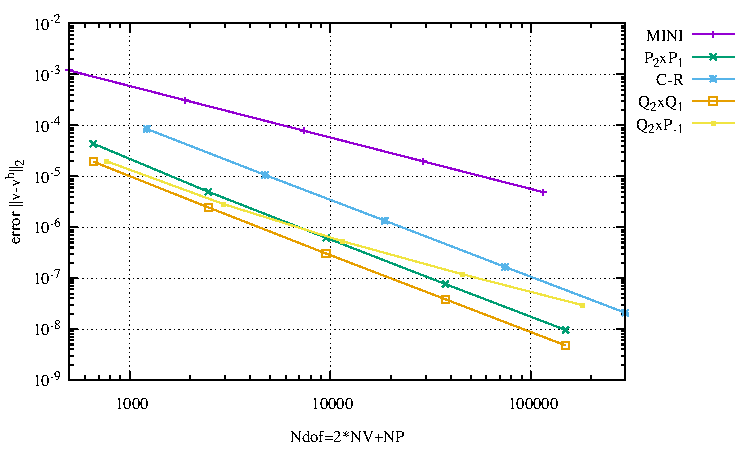
\includegraphics[width=8cm]{python_codes/fieldstone_112/results/exp1_rand/errors_V_ndof.pdf}\\
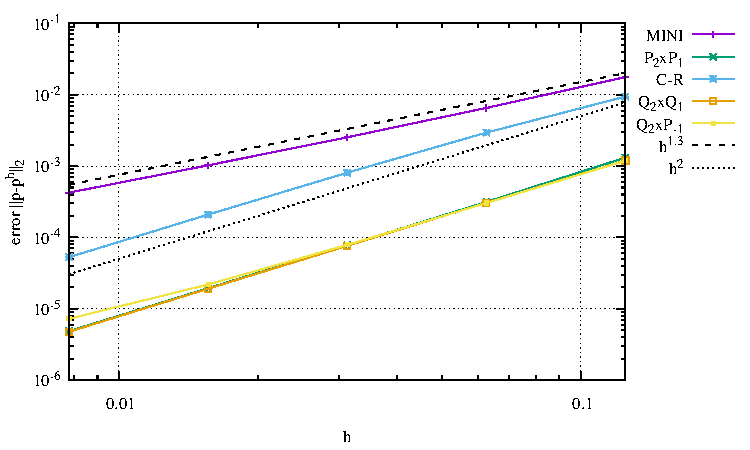
\includegraphics[width=8cm]{python_codes/fieldstone_112/results/exp1_rand/errors_P.pdf}
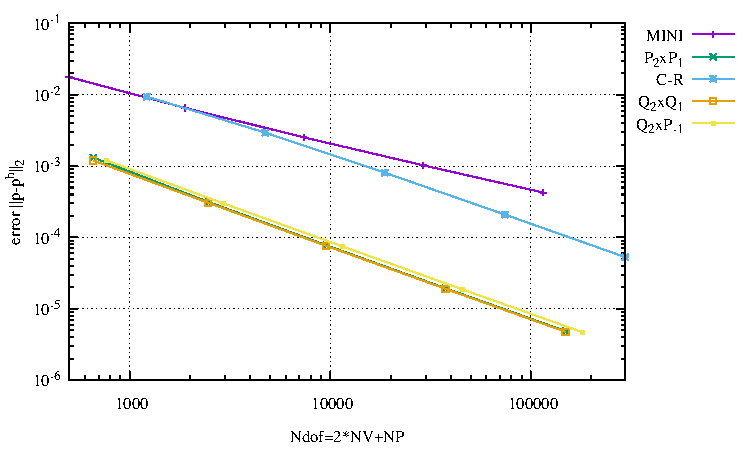
\includegraphics[width=8cm]{python_codes/fieldstone_112/results/exp1_rand/errors_P_ndof.pdf}\\
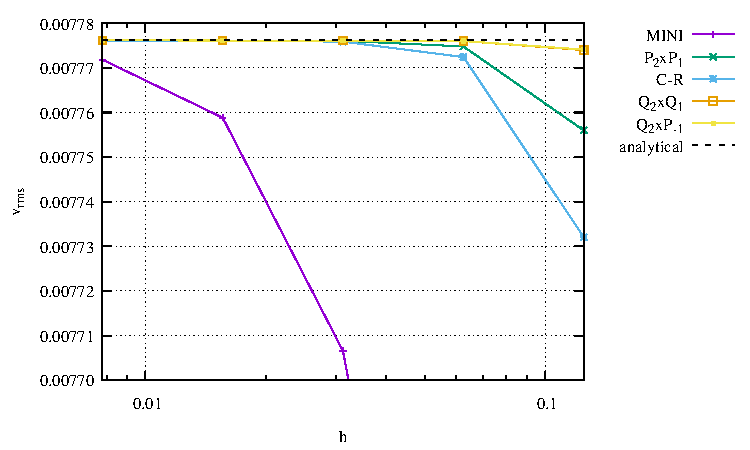
\includegraphics[width=8cm]{python_codes/fieldstone_112/results/exp1_rand/vrms.pdf}
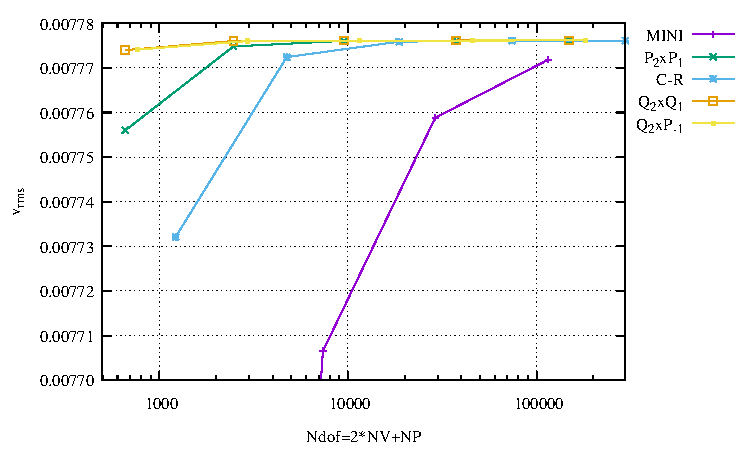
\includegraphics[width=8cm]{python_codes/fieldstone_112/results/exp1_rand/vrms_ndof.pdf}\\
{\captionfont Velocity $L_2$ error (top row), pressure $L_2$ error (middle row) and root
mean square velocity (bottom row) as a function of the element size $h$ (left column) 
and the total number of degrees of freedom (right column).}
\end{center}

\newpage
\begin{center}
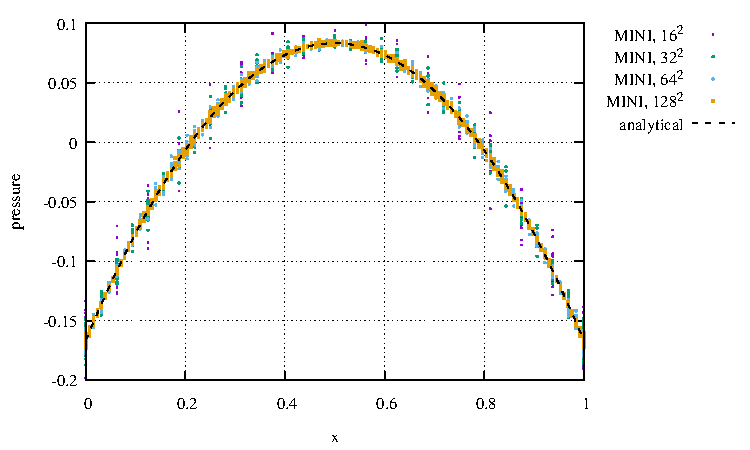
\includegraphics[width=8.5cm]{python_codes/fieldstone_112/results/exp1_rand/pressMINI}
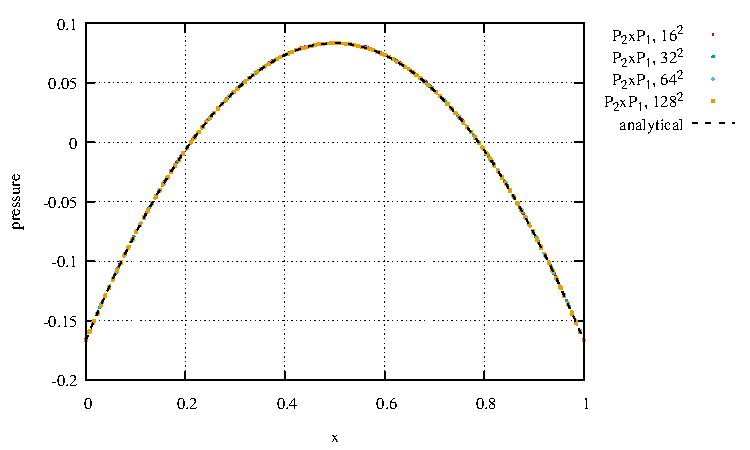
\includegraphics[width=8.5cm]{python_codes/fieldstone_112/results/exp1_rand/pressP2P1}\\
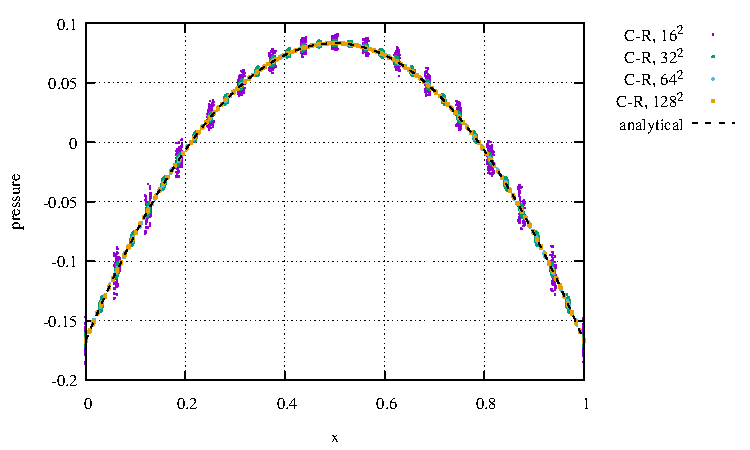
\includegraphics[width=8.5cm]{python_codes/fieldstone_112/results/exp1_rand/pressCR}
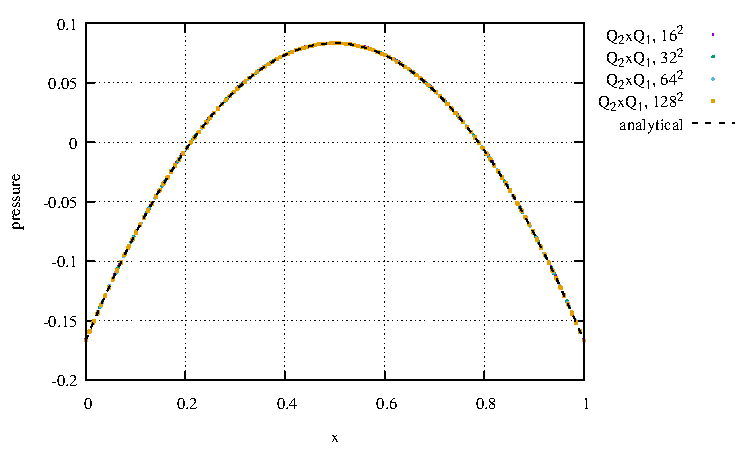
\includegraphics[width=8.5cm]{python_codes/fieldstone_112/results/exp1_rand/pressQ2Q1}\\
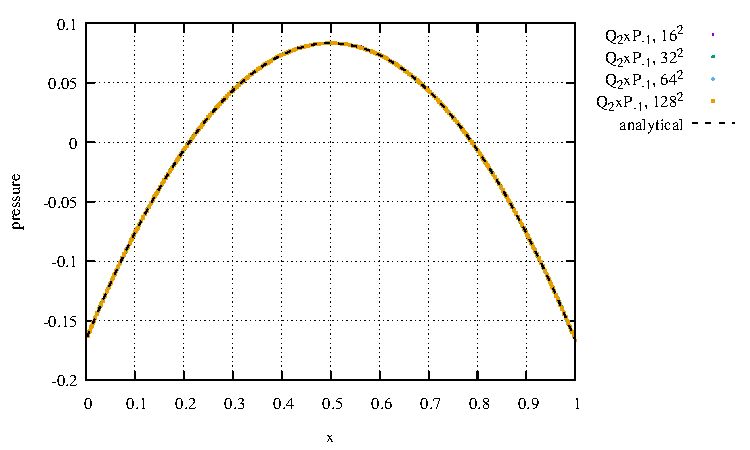
\includegraphics[width=8.5cm]{python_codes/fieldstone_112/results/exp1_rand/pressQ2P1}\\
{\captionfont Pressure field as a function of the $x$-coordinate on a $16\times16$,
$32\times 32$ and $64\times 64$ mesh for all 5 elements.} 
\end{center}

\newpage
%========================================================
\subsection*{Sinking block}

The setup is described in Section~\ref{ss:sinking_block}. No-slip boundary conditions case.
A sinker of size $0.125\times 0.125$ is placed in the middle of the domain. It has density
$\rho=1.01$ while the surrounding fluid has density $\rho=1$. Their respective viscosity is
$\eta=10^3$ and $\eta_1$. Gravity is vertical pointing downwards with $|\vec g|=1$.


\begin{center}
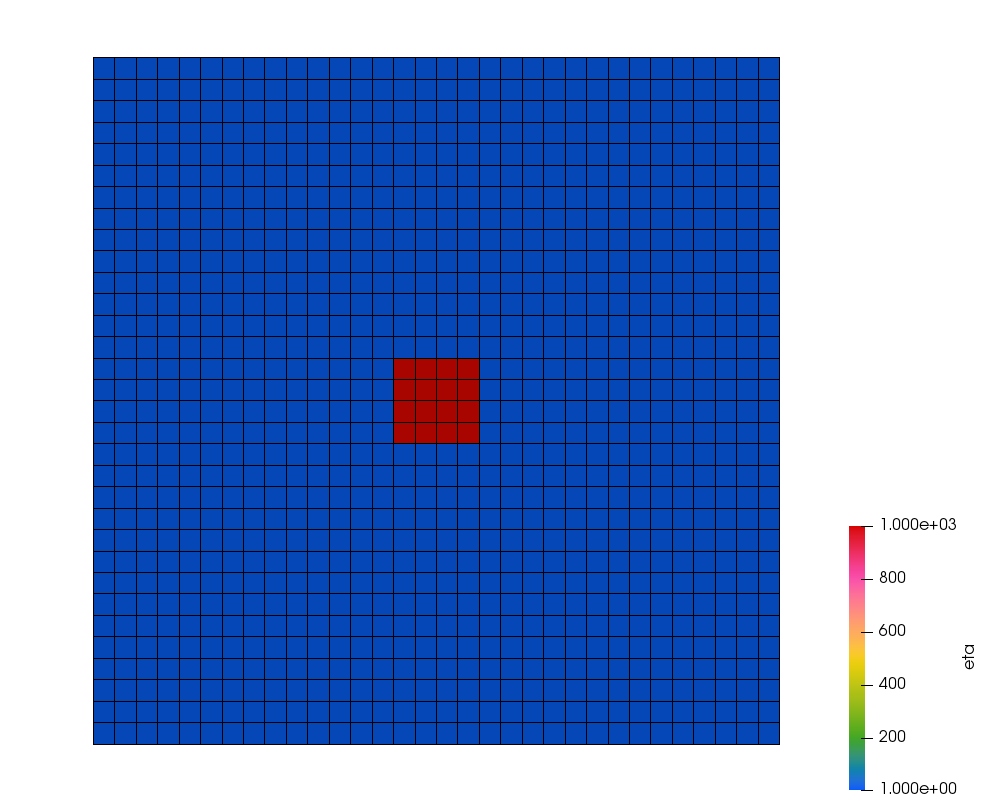
\includegraphics[width=8cm]{python_codes/fieldstone_112/results/exp2/eta}
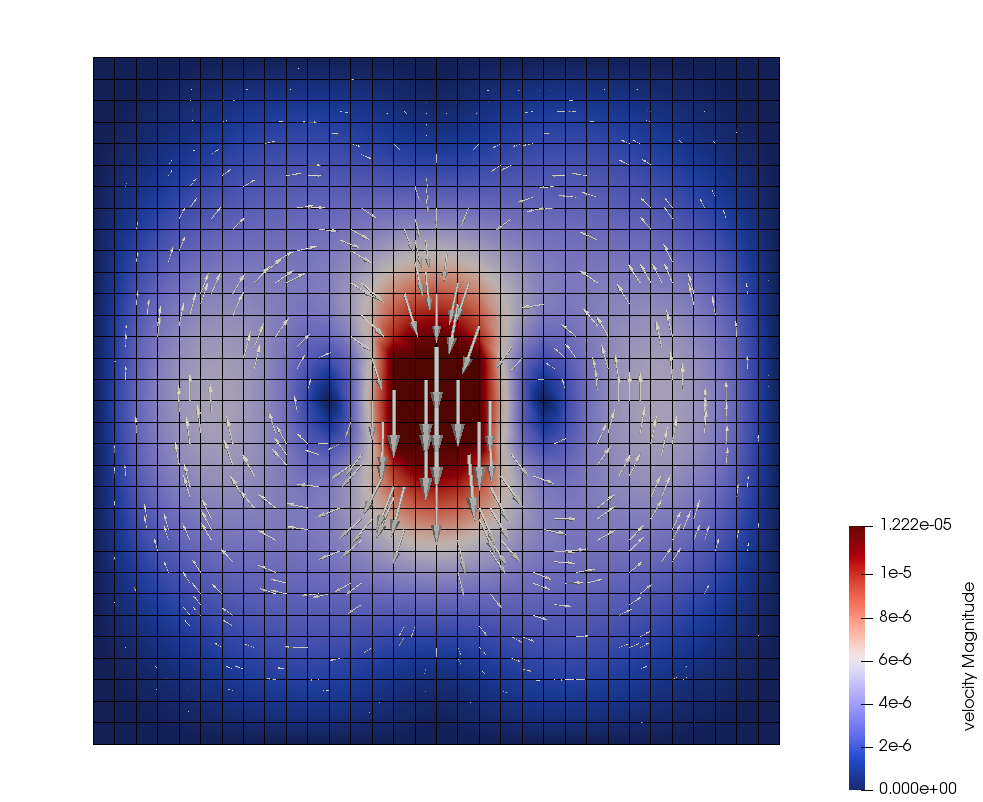
\includegraphics[width=8cm]{python_codes/fieldstone_112/results/exp2/vel}\\
{\captionfont $32\times 32$ grid, $Q_2\times P_{-1}$ element.}
\end{center}

We run this experiment on a $32\times 32$ cell mesh (these cells are then cut in half
in the case of triangular elements). Velocity and pressure are measured on two profiles,
one vertical and one horizontal passing through the middle of the domain.   

\begin{center}
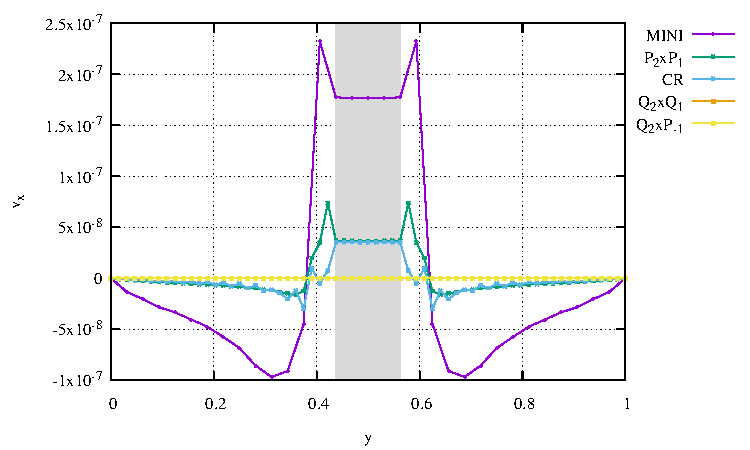
\includegraphics[width=8cm]{python_codes/fieldstone_112/results/exp2/vprofile_u.pdf}
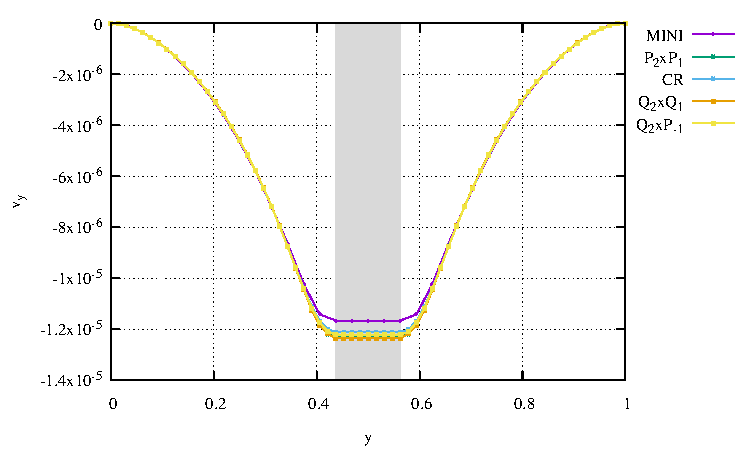
\includegraphics[width=8cm]{python_codes/fieldstone_112/results/exp2/vprofile_v.pdf}\\
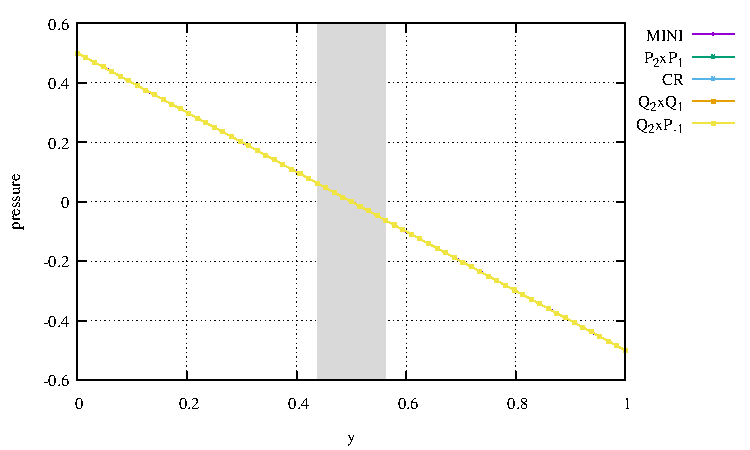
\includegraphics[width=8cm]{python_codes/fieldstone_112/results/exp2/vprofile_p.pdf}
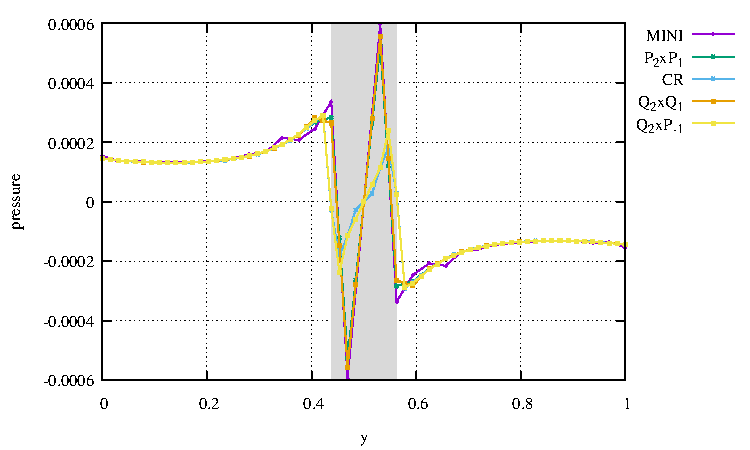
\includegraphics[width=8cm]{python_codes/fieldstone_112/results/exp2/vprofile_pdyn.pdf}\\
{\captionfont Vertical profiles. Pressure is projected onto the velocity nodes.}
\end{center}

\begin{center}
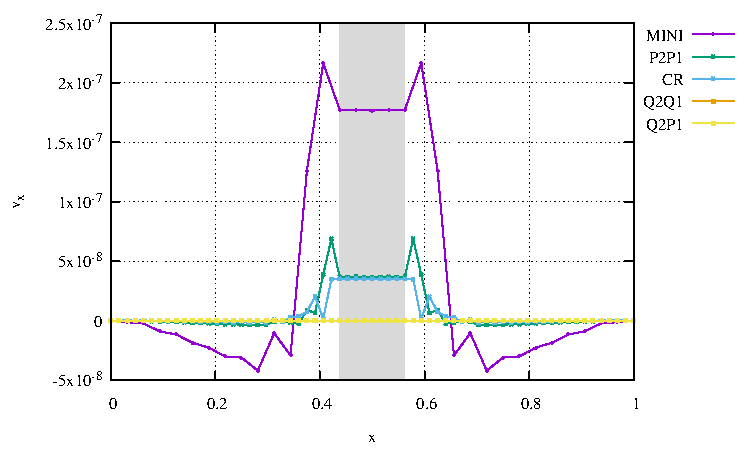
\includegraphics[width=8cm]{python_codes/fieldstone_112/results/exp2/hprofile_u.pdf}
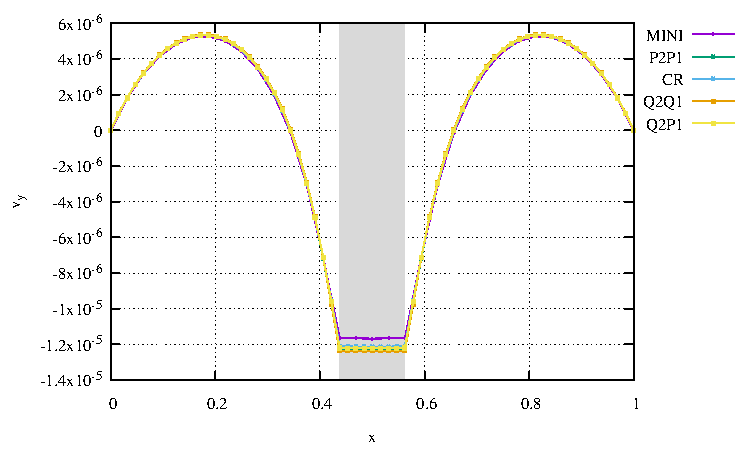
\includegraphics[width=8cm]{python_codes/fieldstone_112/results/exp2/hprofile_v.pdf}
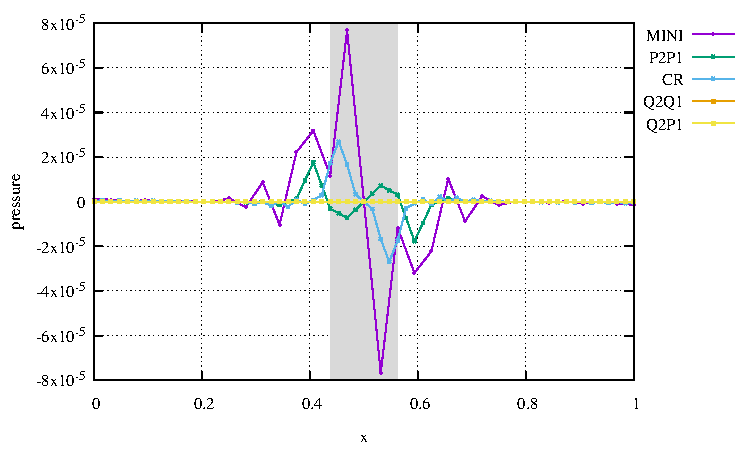
\includegraphics[width=8cm]{python_codes/fieldstone_112/results/exp2/hprofile_p.pdf}\\
{\captionfont Horizontal profiles. Pressure is projected onto the velocity nodes.}
\end{center}

\begin{center}

\includegraphics[height=6cm]{python_codes/fieldstone_112/results/exp2/diag.png}
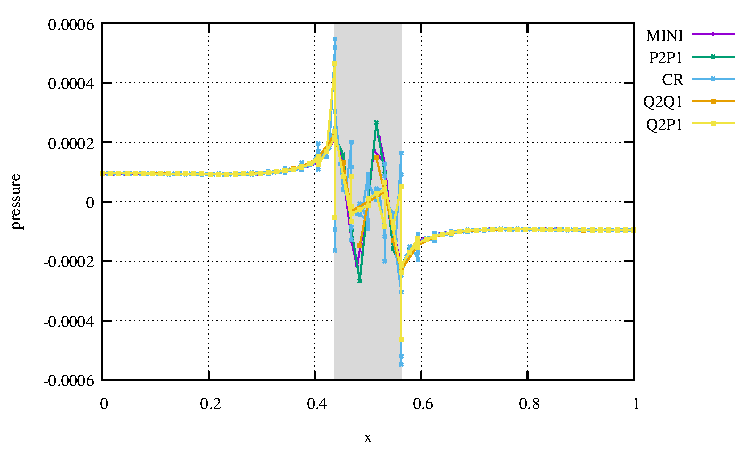
\includegraphics[height=6cm]{python_codes/fieldstone_112/results/exp2/diag_profile_p.pdf}\\
{\captionfont Dynamic pressure $p-p_{lith}$ field on SW-NE diagonal}
\end{center}


\begin{center}
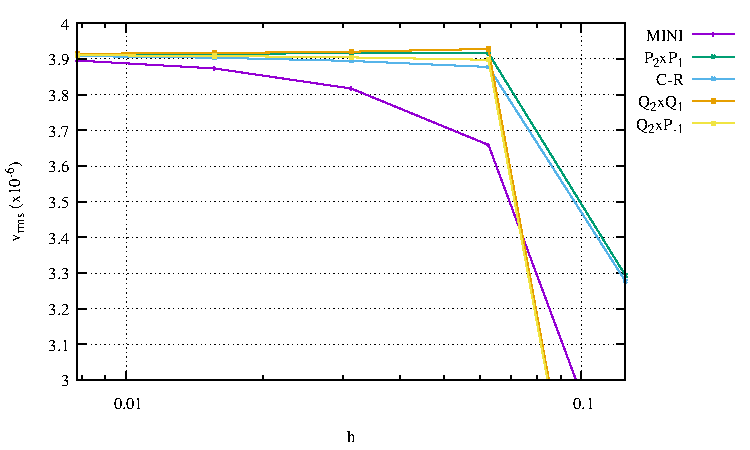
\includegraphics[width=8cm]{python_codes/fieldstone_112/results/exp2/vrms.pdf}
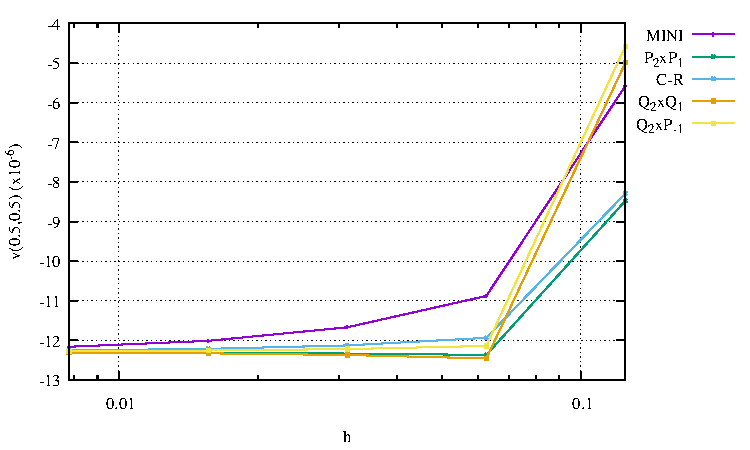
\includegraphics[width=8cm]{python_codes/fieldstone_112/results/exp2/v_center.pdf}\\
{\captionfont Left: root mean square velocity; Right: vertical velocity in the middle of the domain/sinker.}
\end{center}

\newpage
%========================================================
\subsection*{SolCx}

The setup is described in Section~\ref{ss:solcx}. The viscosity is discontinuous 
along the vertical line $x=1/2$ so discontinuous pressure elements perform better:

\begin{center}
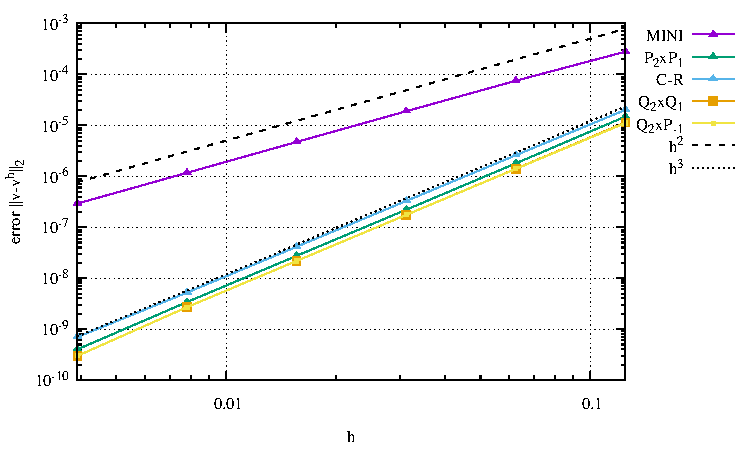
\includegraphics[width=8cm]{python_codes/fieldstone_112/results/exp3/errors_V.pdf}
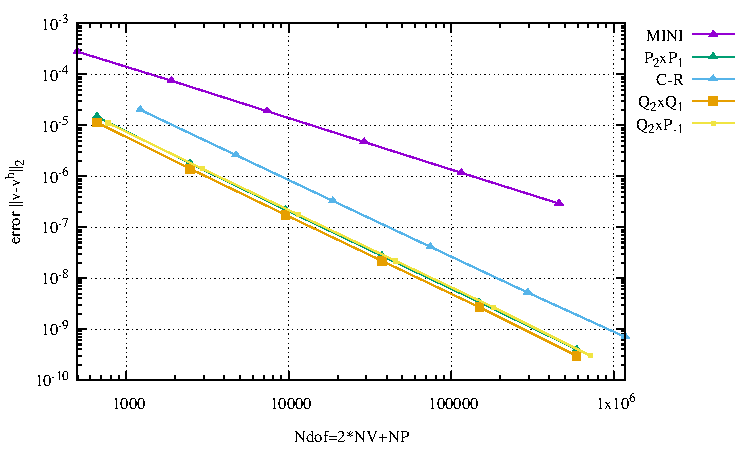
\includegraphics[width=8cm]{python_codes/fieldstone_112/results/exp3/errors_V_ndof.pdf}\\
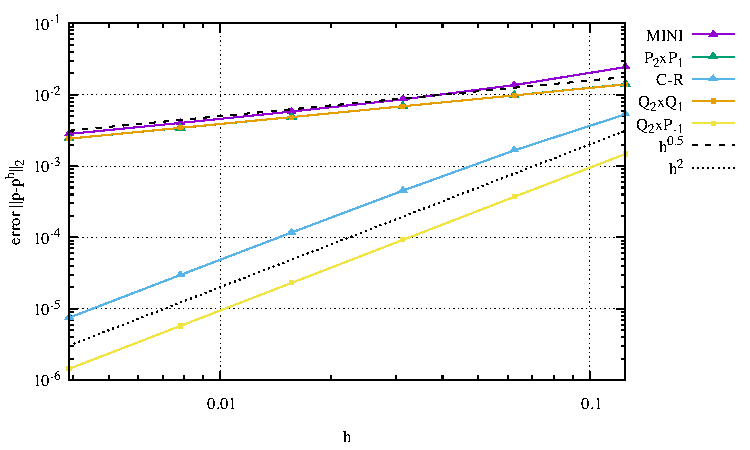
\includegraphics[width=8cm]{python_codes/fieldstone_112/results/exp3/errors_P.pdf}
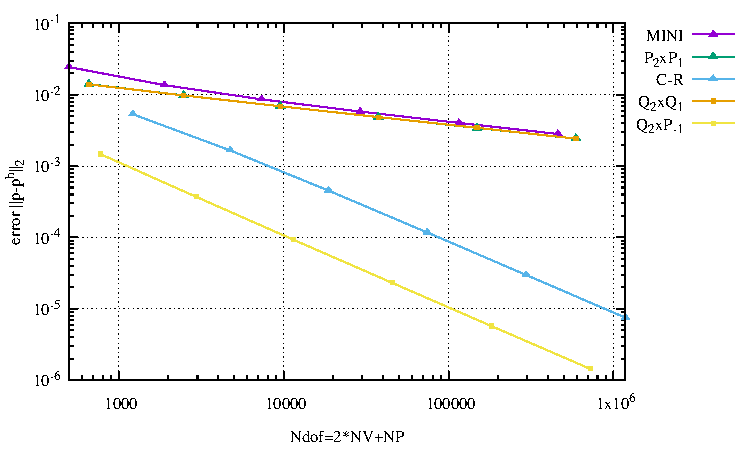
\includegraphics[width=8cm]{python_codes/fieldstone_112/results/exp3/errors_P_ndof.pdf}\\
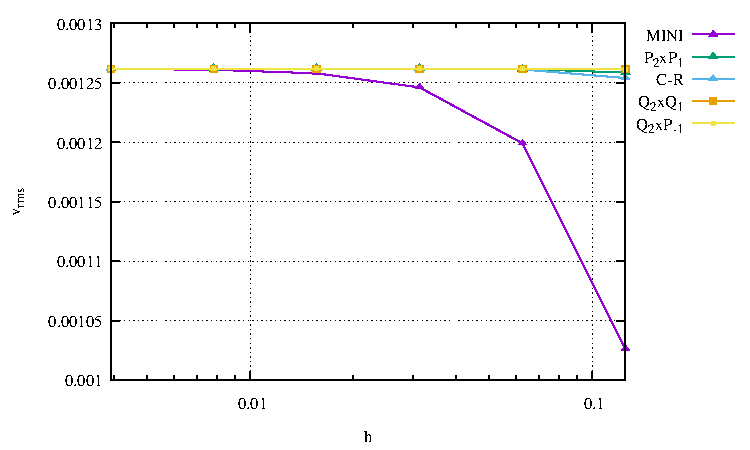
\includegraphics[width=8cm]{python_codes/fieldstone_112/results/exp3/vrms.pdf}
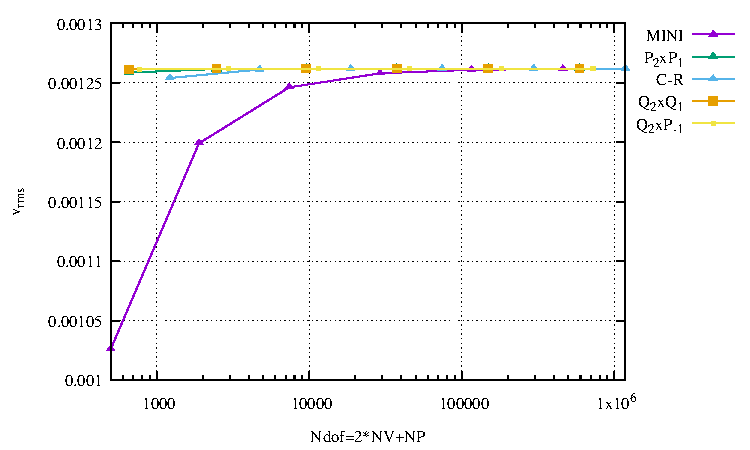
\includegraphics[width=8cm]{python_codes/fieldstone_112/results/exp3/vrms_ndof.pdf}\\
{\captionfont Velocity $L_2$ error (top row), pressure $L_2$ error (middle row) and vrms (bottom row) 
as a function of the element size $h$ (left column) and the total number of dofs (right column).}
\end{center}

Thieulot \& Bangerth (2021) \cite{thba21} report ${\cal O}(h^3)$ for velocity for both $Q_2\times Q_1$ and $Q_2\times P_1$
and ${\cal O}(h^{0.5})$ for $Q_2\times Q_1$ and  ${\cal O}(h^{2})$ for $Q_2\times P_{-1}$ for pressure. 
Our measurements are similar here.

\newpage
%========================================================
\subsection*{SolKz}

The setup is described in Section~\ref{ss:solkz}. 

\begin{center}
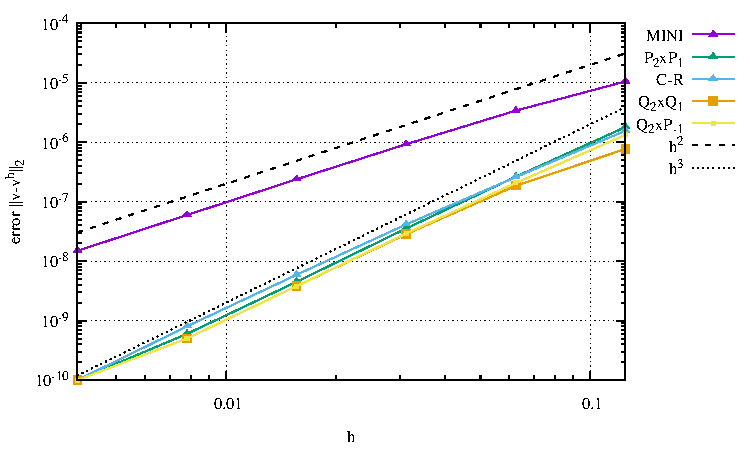
\includegraphics[width=8cm]{python_codes/fieldstone_112/results/exp4/errors_V.pdf}
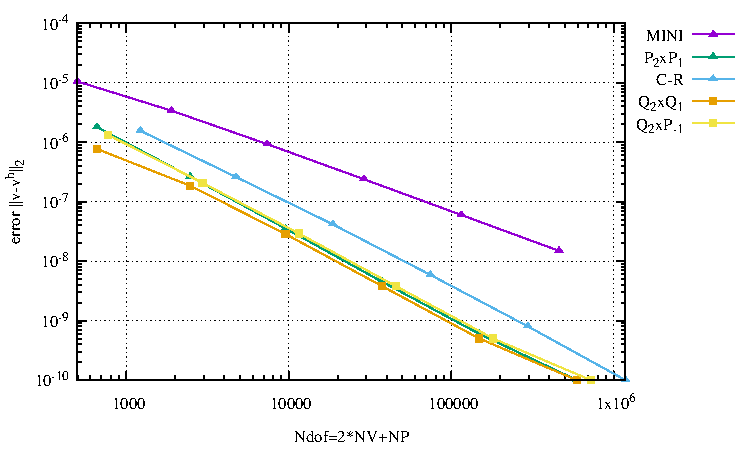
\includegraphics[width=8cm]{python_codes/fieldstone_112/results/exp4/errors_V_ndof.pdf}\\
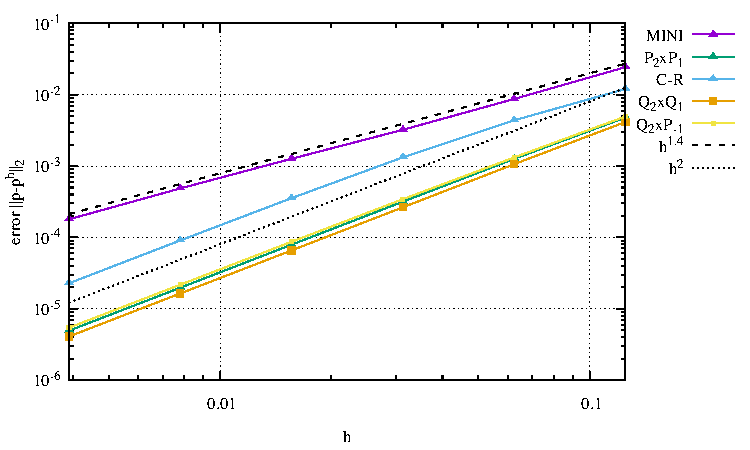
\includegraphics[width=8cm]{python_codes/fieldstone_112/results/exp4/errors_P.pdf}
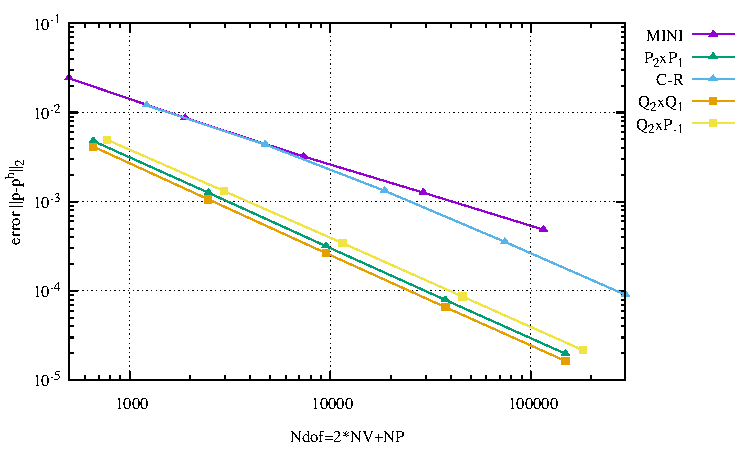
\includegraphics[width=8cm]{python_codes/fieldstone_112/results/exp4/errors_P_ndof.pdf}\\
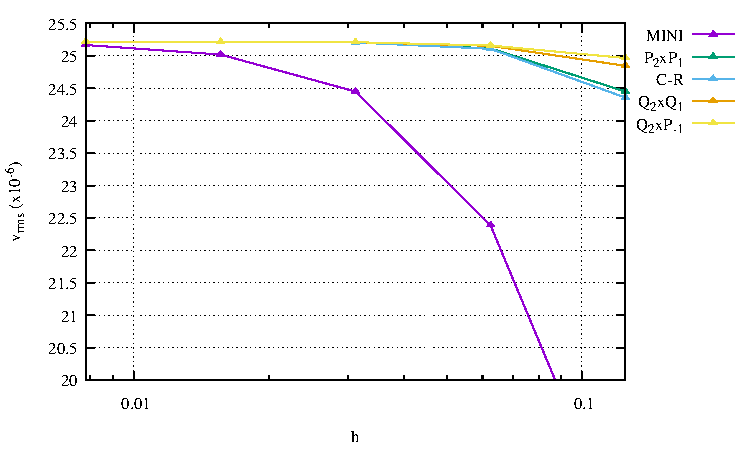
\includegraphics[width=8cm]{python_codes/fieldstone_112/results/exp4/vrms.pdf}
\includegraphics[width=8cm]{python_codes/fieldstone_112/results/exp4/vrms_ndof.pdf}\\
{\captionfont Velocity $L_2$ error (top row), pressure $L_2$ error (middle row) and vrms (bottom row) 
as a function of the element size $h$ (left column) and the total number of dofs (right column).}
\end{center}

Note the 1.4 convergence of pressure for MINI

\newpage
Influence of mesh quality: A random perturbation is added to the interior nodes. 

\begin{center}
\includegraphics[width=8cm]{python_codes/fieldstone_112/results/exp4_rand/errors_V.pdf}
\includegraphics[width=8cm]{python_codes/fieldstone_112/results/exp4_rand/errors_V_ndof.pdf}\\
\includegraphics[width=8cm]{python_codes/fieldstone_112/results/exp4_rand/errors_P.pdf}
\includegraphics[width=8cm]{python_codes/fieldstone_112/results/exp4_rand/errors_P_ndof.pdf}\\
\includegraphics[width=8cm]{python_codes/fieldstone_112/results/exp4_rand/vrms.pdf}
\includegraphics[width=8cm]{python_codes/fieldstone_112/results/exp4_rand/vrms_ndof.pdf}\\
{\captionfont Velocity $L_2$ error (top row), pressure $L_2$ error (middle row) and root
mean square velocity (bottom row) as a function of the element size $h$ (left column) 
and the total number of degrees of freedom (right column).}
\end{center}





\newpage
%========================================================
\subsection*{SolVi}

The setup is described in Section~\ref{ss:solvi}. 

\begin{center}
\includegraphics[width=8cm]{python_codes/fieldstone_112/results/exp5/errors_V.pdf}
\includegraphics[width=8cm]{python_codes/fieldstone_112/results/exp5/errors_V_ndof.pdf}\\
\includegraphics[width=8cm]{python_codes/fieldstone_112/results/exp5/errors_P.pdf}
\includegraphics[width=8cm]{python_codes/fieldstone_112/results/exp5/errors_P_ndof.pdf}\\
\includegraphics[width=8cm]{python_codes/fieldstone_112/results/exp5/vrms.pdf}
\includegraphics[width=8cm]{python_codes/fieldstone_112/results/exp5/vrms_ndof.pdf}\\
{\captionfont Velocity $L_2$ error (top row), pressure $L_2$ error (middle row) and vrms (bottom row) 
as a function of the element size $h$ (left column) and the total number of dofs (right column).}
\end{center}

Thieulot \& Bangerth (2021) \cite{thba21} report ${\cal O}(h)$ convergence for 
velocity and ${\cal O}(h^{0.5})$ for pressure across all four elements that they tested.
Our measurements are similar here.


\begin{center}
\includegraphics[width=8.5cm]{python_codes/fieldstone_112/results/exp5/bottom64}
\includegraphics[width=8.5cm]{python_codes/fieldstone_112/results/exp5/bottom128}\\
{\captionfont Pressure at the bottom of the domain. Grey area corresponds to the 
high viscosity disc. Left: 64x64 cells; right: 128x128 cells.}
\end{center}

\newpage
%===================================================================================
\subsection*{SolVi - A quick look at how viscosity is prescribed}

The interface between the inclusion and the matrix is never aligned with 
element edges so that inside the elements cut by this interface some 
quadrature points are assigned $\eta_q=\eta_{i}=10^3$ and other 
quadrature points are assigned $\eta_q=\eta_{m}=1$. 

It is well known that such an approach often yields less accurate results
than when the viscosity in the element is either constant or linear (see 
current work by Gerry and also \aspect manual).

In order to avoid the discussion of which averaging is best suited, 
I have simply here explored the possibility of assigning a constant 
viscosity inside each element based on whether or not its barycenter is 
inside or outside the inclusion.

\begin{center}
\includegraphics[width=8cm]{python_codes/fieldstone_112/results/exp5_avrg/errors_V.pdf}
\includegraphics[width=8cm]{python_codes/fieldstone_112/results/exp5_avrg/errors_V_ndof.pdf}\\
\includegraphics[width=8cm]{python_codes/fieldstone_112/results/exp5_avrg/errors_P.pdf}
\includegraphics[width=8cm]{python_codes/fieldstone_112/results/exp5_avrg/errors_P_ndof.pdf}\\
\includegraphics[width=8cm]{python_codes/fieldstone_112/results/exp5_avrg/vrms.pdf}
\includegraphics[width=8cm]{python_codes/fieldstone_112/results/exp5_avrg/vrms_ndof.pdf}\\
{\captionfont Velocity $L_2$ error (top row), pressure $L_2$ error (middle row) and vrms (bottom row) 
as a function of the element size $h$ (left column) and the total number of dofs (right column).
Dashed lines correspond to the reference case (see previous section) while continuous lines
correspond to elemental viscosities. }
\end{center}
 
We find that results seem to be more accurate but the convergence rates for both 
velocity and pressure are not significantly improved.


\newpage
%===================================================================================
\subsection*{SolVi - focus on triangular elements and how quadrilaterals are split}
The mesh consists of $nelx \times nely$ cells. When triangular elements are used, 
each quadrilateral cell can be split either along one diagonal or the other. 
There are then three options in the code: if {\tt tridiag}=0, then all cells are split 
along the NW-SE diagonal, if {\tt tridiag}=1, then all cells are split
along the SW-NE diagonal, and if {\tt tridiag}=2, then cells are split 
randomly across one or the other diagonal, as shown in the following figure:

\begin{center}
\includegraphics[width=4.5cm]{python_codes/fieldstone_112/results/exp5_tridiag/tridiag0}
\includegraphics[width=4.5cm]{python_codes/fieldstone_112/results/exp5_tridiag/tridiag1}
\includegraphics[width=4.5cm]{python_codes/fieldstone_112/results/exp5_tridiag/tridiag2}\\
{\captionfont From left to right: tridiag=0,1,2. 16x16 cells.}
\end{center}

\begin{center}

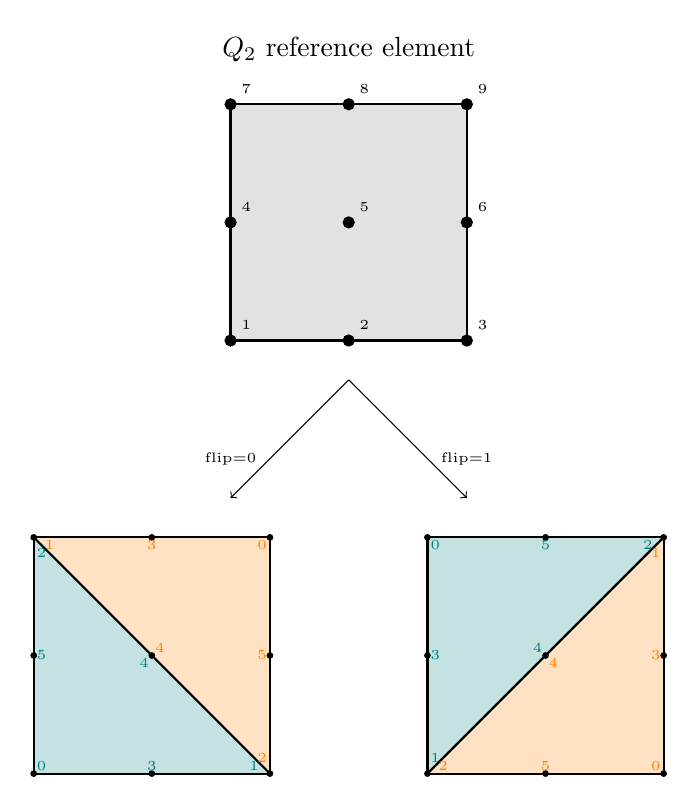
\begin{tikzpicture}
%\draw[fill=gray!23,gray!23](0,0) rectangle (9,10);
%\draw[step=0.5cm,gray,very thin] (0,0) grid (9,10); %background grid

\draw[fill=teal!23,teal!23](0.5,0.5) -- (3.5,0.5) -- (0.5,3.5) -- cycle;
\draw[fill=orange!23,orange!23](3.5,0.5) --(3.5,3.5) -- (0.5,3.5) -- cycle;
\draw[thick] (0.5,0.5) -- (3.5,0.5) -- (3.5,3.5) -- (0.5,3.5) -- cycle; %left
\draw[thick] (0.5,3.5) -- (3.5,0.5) ;
\draw[black,fill=black] (0.5,0.5)   circle (1pt);
\draw[black,fill=black] (2,0.5)   circle (1pt);
\draw[black,fill=black] (3.5,0.5)   circle (1pt);
\draw[black,fill=black] (0.5,2)   circle (1pt);
\draw[black,fill=black] (2,2)   circle (1pt);
\draw[black,fill=black] (3.5,2)   circle (1pt);
\draw[black,fill=black] (0.5,3.5)   circle (1pt);
\draw[black,fill=black] (2,3.5)   circle (1pt);
\draw[black,fill=black] (3.5,3.5)   circle (1pt);
\node[] at (0.6,0.6) {\tiny \color{teal} 0};
\node[] at (2,0.6) {\tiny \color{teal} 3};
\node[] at (3.3,0.6) {\tiny \color{teal} 1};
\node[] at (0.6,2) {\tiny \color{teal} 5};
\node[] at (1.9,1.9) {\tiny \color{teal} 4};
\node[] at (0.6,3.3) {\tiny \color{teal} 2};
\node[] at (3.4,3.4) {\tiny \color{orange} 0};
\node[] at (2,3.4) {\tiny \color{orange} 3};
\node[] at (0.7,3.4) {\tiny \color{orange} 1};
\node[] at (3.4,2) {\tiny \color{orange} 5};
\node[] at (3.4,0.7) {\tiny \color{orange} 2};
\node[] at (2.1,2.1) {\tiny \color{orange} 4};



\draw[fill=teal!23,teal!23](5.5,0.5) -- (8.5,3.5) -- (5.5,3.5) -- cycle;
\draw[fill=orange!23,orange!23](5.5,0.5) --(8.5,0.5) -- (8.5,3.5) -- cycle;

\draw[thick] (5.5,0.5) -- (8.5,0.5) -- (8.5,3.5) -- (5.5,3.5) -- cycle; %right
\draw[thick] (5.5,0.5) -- (8.5,3.5) ;
\draw[black,fill=black] (5.5,0.5)   circle (1pt);
\draw[black,fill=black] (7,0.5)   circle (1pt);
\draw[black,fill=black] (8.5,0.5)   circle (1pt);
\draw[black,fill=black] (5.5,2)   circle (1pt);
\draw[black,fill=black] (7,2)   circle (1pt);
\draw[black,fill=black] (8.5,2)   circle (1pt);
\draw[black,fill=black] (5.5,3.5)   circle (1pt);
\draw[black,fill=black] (7,3.5)   circle (1pt);
\draw[black,fill=black] (8.5,3.5)   circle (1pt);
\node[] at (8.4,0.6) {\tiny \color{orange} 0};
\node[] at (8.4,2) {\tiny \color{orange} 3};
\node[] at (8.4,3.3) {\tiny \color{orange} 1};
\node[] at (7,0.6) {\tiny \color{orange} 5};
\node[] at (7.1,1.9) {\tiny \color{orange} 4};
\node[] at (5.7,0.6) {\tiny \color{orange} 2};

\node[] at (5.6,3.4) {\tiny \color{teal} 0};
\node[] at (5.6,2) {\tiny \color{teal} 3};
\node[] at (5.6,0.7) {\tiny \color{teal} 1};
\node[] at (7,3.4) {\tiny \color{teal} 5};
\node[] at (6.9,2.1) {\tiny \color{teal} 4};
\node[] at (8.3,3.4) {\tiny \color{teal} 2};

\draw[thin,->] (4.5,5.5) -- (3,4); 
\draw[thin,->] (4.5,5.5) -- (6,4); 
\node[] at (3,4.5) {\tiny flip=0};
\node[] at (6,4.5) {\tiny flip=1};

\node[] at (4.5,9.7) {$Q_2$ reference element};
\draw[fill=gray!23,gray!23](3,6) rectangle (6,9);
\draw[thick] (3,6) -- (6,6) -- (6,9) -- (3,9) -- cycle; %top
\draw[black,fill=black] (3,6)   circle (2pt);
\draw[black,fill=black] (4.5,6)   circle (2pt);
\draw[black,fill=black] (6,6)   circle (2pt);
\draw[black,fill=black] (3,7.5)   circle (2pt);
\draw[black,fill=black] (4.5,7.5)   circle (2pt);
\draw[black,fill=black] (6,7.5)   circle (2pt);
\draw[black,fill=black] (3,9)   circle (2pt);
\draw[black,fill=black] (4.5,9)   circle (2pt);
\draw[black,fill=black] (6,9)   circle (2pt);
\node[] at (3.2,6.2) {\tiny 1};
\node[] at (4.7,6.2) {\tiny 2};
\node[] at (6.2,6.2) {\tiny 3};
\node[] at (3.2,7.7) {\tiny 4};
\node[] at (4.7,7.7) {\tiny 5};
\node[] at (6.2,7.7) {\tiny 6};
\node[] at (3.2,9.2) {\tiny 7};
\node[] at (4.7,9.2) {\tiny 8};
\node[] at (6.2,9.2) {\tiny 9};

\end{tikzpicture}



{\captionfont How the biquadratic quadrilateral is split into two quadratic triangles. 
Numbers correspond to internal numbering.}
\end{center}

\vspace{1cm}

\begin{center}
\includegraphics[width=5.5cm]{python_codes/fieldstone_112/results/exp5_tridiag/64x64_tridiag1/MINI}
\includegraphics[width=5.5cm]{python_codes/fieldstone_112/results/exp5_tridiag/64x64_tridiag1/P2P1}
\includegraphics[width=5.5cm]{python_codes/fieldstone_112/results/exp5_tridiag/64x64_tridiag1/CR}\\
{\captionfont From left to right: pressure field obtained with MINI, P2P1 and CR elements on 64x64 mesh
with SE-NW splitting.}
\end{center}



\newpage
The following plot are similar to those before but each element/resolution combination is (\textit{still}) being run 
250 times so as to generate 250 different meshes with different random cell splits. The important conclusion
are that a) the maximum of the error across the 250 meshes converges faster for the pressure than for velocity
up to about $100\times 100$ resolutions b) it then takes converges at a lower rate, i.e. $\propto h^{0.5}$. 

Resolutions on the following plots range from 8x8 to 200x200. I will run up to 300x300 during the xmas break.

\begin{center}
\includegraphics[width=5.7cm]{python_codes/fieldstone_112/results/exp5_tridiag/errors_V_MINI.pdf}
\includegraphics[width=5.7cm]{python_codes/fieldstone_112/results/exp5_tridiag/errors_V_P2P1.pdf}
\includegraphics[width=5.7cm]{python_codes/fieldstone_112/results/exp5_tridiag/errors_V_CR.pdf}\\
\includegraphics[width=5.7cm]{python_codes/fieldstone_112/results/exp5_tridiag/errors_P_MINI.pdf}
\includegraphics[width=5.7cm]{python_codes/fieldstone_112/results/exp5_tridiag/errors_P_P2P1.pdf}
\includegraphics[width=5.7cm]{python_codes/fieldstone_112/results/exp5_tridiag/errors_P_CR.pdf}\\
{\captionfont Velocity (top row) and pressure (bottom row) error as a function of the element size
for the MINI (left), $P_2\times P_1$ (middle) and C-R element (right).}
\end{center}



\begin{center}
\includegraphics[width=8cm]{python_codes/fieldstone_112/results/exp5_tridiag/errors_V_ndof.pdf}
\includegraphics[width=8cm]{python_codes/fieldstone_112/results/exp5_tridiag/errors_P_ndof.pdf}\\
{\captionfont Velocity $L_2$ error (left), pressure $L_2$ error (right) as a function of the total 
number of degrees of freedom.} 
\end{center}


\begin{center}
\includegraphics[width=8cm]{python_codes/fieldstone_112/results/exp5_tridiag/vrms.pdf}
\includegraphics[width=8cm]{python_codes/fieldstone_112/results/exp5_tridiag/vrms_ndof.pdf}\\
{\captionfont vrms as a function of the element size $h$ (left) and the total number of dofs (right).}
\end{center}


\newpage
%========================================================
\subsection*{SolVg (Viscosity grooves)}

This manufactured solution is presented in Section~\ref{mms7} and is also implemented in \aspect.
Domain is 2x2. The $\epsilon$ parameter controls the viscosity amplitude and is set to 0.001.

\begin{center}
\includegraphics[width=5cm]{python_codes/fieldstone_112/results/exp6/vel}
\includegraphics[width=5cm]{python_codes/fieldstone_112/results/exp6/press}
\includegraphics[width=5cm]{python_codes/fieldstone_112/results/exp6/eta}\\
{\captionfont Velocity, pressure and (elemental) viscosity field for $\epsilon=0.001$ on a 64x64 mesh}
\end{center}


\begin{center}
\includegraphics[width=8cm]{python_codes/fieldstone_112/results/exp6/errors_V.pdf}
\includegraphics[width=8cm]{python_codes/fieldstone_112/results/exp6/errors_V_ndof.pdf}\\
\includegraphics[width=8cm]{python_codes/fieldstone_112/results/exp6/errors_P.pdf}
\includegraphics[width=8cm]{python_codes/fieldstone_112/results/exp6/errors_P_ndof.pdf}\\
\includegraphics[width=8cm]{python_codes/fieldstone_112/results/exp6/vrms.pdf}
\includegraphics[width=8cm]{python_codes/fieldstone_112/results/exp6/vrms_ndof.pdf}\\
{\captionfont Velocity $L_2$ error (top row), pressure $L_2$ error (middle row) and vrms (bottom row) 
as a function of the element size $h$ (left column) and the total number of dofs (right column).}
\end{center}






%%%%%%%%%%%%%%%%%%%%%%%%%%%%%%%%%%%%%%%%%%%%%%%%%%%%%%%%%%%%%%%%%%%%%%%%%%%%%%%%%%%
%%%%%%%%%%%%%%%%%%%%%%%%%%%%%%%%%%%%%%%%%%%%%%%%%%%%%%%%%%%%%%%%%%%%%%%%%%%%%%%%%%%
%%%%%%%%%%%%%%%%%%%%%%%%%%%%%%%%%%%%%%%%%%%%%%%%%%%%%%%%%%%%%%%%%%%%%%%%%%%%%%%%%%%
\newpage




Assuming that $
\| {\bm u} - {\bm u}_h \|_{L_2} = {\cal O}(h^{\alpha_v})
$ and $
\| p - p_h \|_{L_2} = {\cal O}(h^{\alpha_p})
$
I have gathered the exponent values in the following 
table. 


\begin{tabular}{|l|llll|llll|llll|llll|llll|}
\hline
& 
\multicolumn{4}{c|}{MINI}&  
\multicolumn{4}{c|}{$P_2\times P_1$}  & 
\multicolumn{4}{c|}{C-R}  & 
\multicolumn{4}{c|}{$Q_2\times Q_1$} &  
\multicolumn{4}{c|}{$Q_2\times P_1$}  \\
experiment      & 
$\alpha_v$ & r  &  $\alpha_p$ & r &  
$\alpha_v$ & r  &  $\alpha_p$ & r &  
$\alpha_v$ & r  &  $\alpha_p$ & r &  
$\alpha_v$ & r  & $\alpha_p$ & r &   
$\alpha_v$ & r  & $\alpha_p$ & r \\
\hline
\hline
D \& H 
&{2}&4&1.5&3
&{3}&2&2&1
&{3}&3&2&2
&{3}&1&2&1
&{3}&1&2&1\\
D \& H (rand)
&2&5&1.3&3
&3&2&2&1
&3&3&2&2
&3&1&2&1
&3&1&2&1 \\
SolCx 
&2&4&0.5&4
&3&2&0.5&3
&3&3&2&2
&3&1&0.5&3
&3&1&2&1\\
SolKz 
&2&4&1.4&5
&3&2&2&2
&3&3&2&4
&3&1&2&1
&3&1&2&3\\
SolKz (rand)
&2&4&1.2&5
&3&2&2&2
&3&3&2&4
&3&1&2&1
&3&1&2&3\\
SolVi 
&1&-&0.5&3
&1&-&0.5&1
&1&-&0.5&4
&1&-&0.5&2
&1&-&0.5&5\\
SolVi (multi) \\ 
SolVg &
2&4&1.15&4&
3&2&2&2&
3&3&2&3&
3&1&2&1&
3&1&2&2\\
\hline
total  
&-&?&-&?
&-&?&-&?
&-&?&-&?
&-&?&-&?
&-&?&-&?\\
\hline
\end{tabular}

The r value corresponds to the \textbf{r}anking. For instance if Q2Q1 is the most accurate for velocity on D \& H then it gets a 1, then P2P1 gets a 2 because it was the second best accurate element, etc ...
In the end I would sum all the $r$ values per column (replacing the '?') 
and the smaller the value the better the element. 

Note that SolVi measurements will be updated when all the runs have completed.  







%========================================================
\subsection*{Preliminary Conclusions}

\begin{itemize}
\item the MINI element is very appealing (a single bubble added to $P_1$) and cheap. However it is also 
the least accurate element, even looking at the errors as function of number of dofs and not $h$
\item P2P1 always more accurate than CR except for SolCx where disc pressure elements are way more accurate.
\item P2P1 about as accurate as Q2Q1 in all benchmarks
\end{itemize}


%========================================================
\subsection*{Open questions}

\begin{itemize}
%\item what is a good measure $h$ for triangles in general ? sqrt of area ? hypothenuse ? min of edges length? 
\item at the moment I build the entire Stokes matrix in a sparse format and send it to the default 
python solver. This means that no iterative solver is used (inner or outer) so that the discussion 
on the nb of FGMRES iterations of our paper cannot be carried out here. 
\item Right now viscosity is computed on quadrature point. No averaging. It probably only really matters 
for SolVi and SolVg (and may be a bit for SolKz). Should I implement elemental averaging and try?  
\item are there other elements you wish to add to this list? $P_3\times P_2$ ? 
\item I plot now the velocity and pressure errors as a function of the total number of dofs. 
Does this make sense? or should I plot the velocity errors as a fct of the velocity dofs and 
the pressure errors  as a fct of pressure dofs?
\item any thoughts about my ranking system ?like it ? hate it ?
\item am I right to think that $Q_2\times P_{-1}$ in \aspect is of the unmapped type ?  (\textcite{boga02} (2002))
\item should I repeat the same statistical study with 250 different triangular meshes per element for SolVg ? 
\end{itemize}

\vspace{0.5cm}

note to myself: check and probably remove stone 46, 47 ?
